\documentclass[12pt,modern]{article}
\usepackage{fancyhdr}
\usepackage{graphicx}
\usepackage[margin=1in]{geometry}

\pagestyle{fancy}
\fancyhf{}
\lhead{AU Mic Research Overview}
\rhead{Cail Daley}

\begin{document}

\begin{figure}
  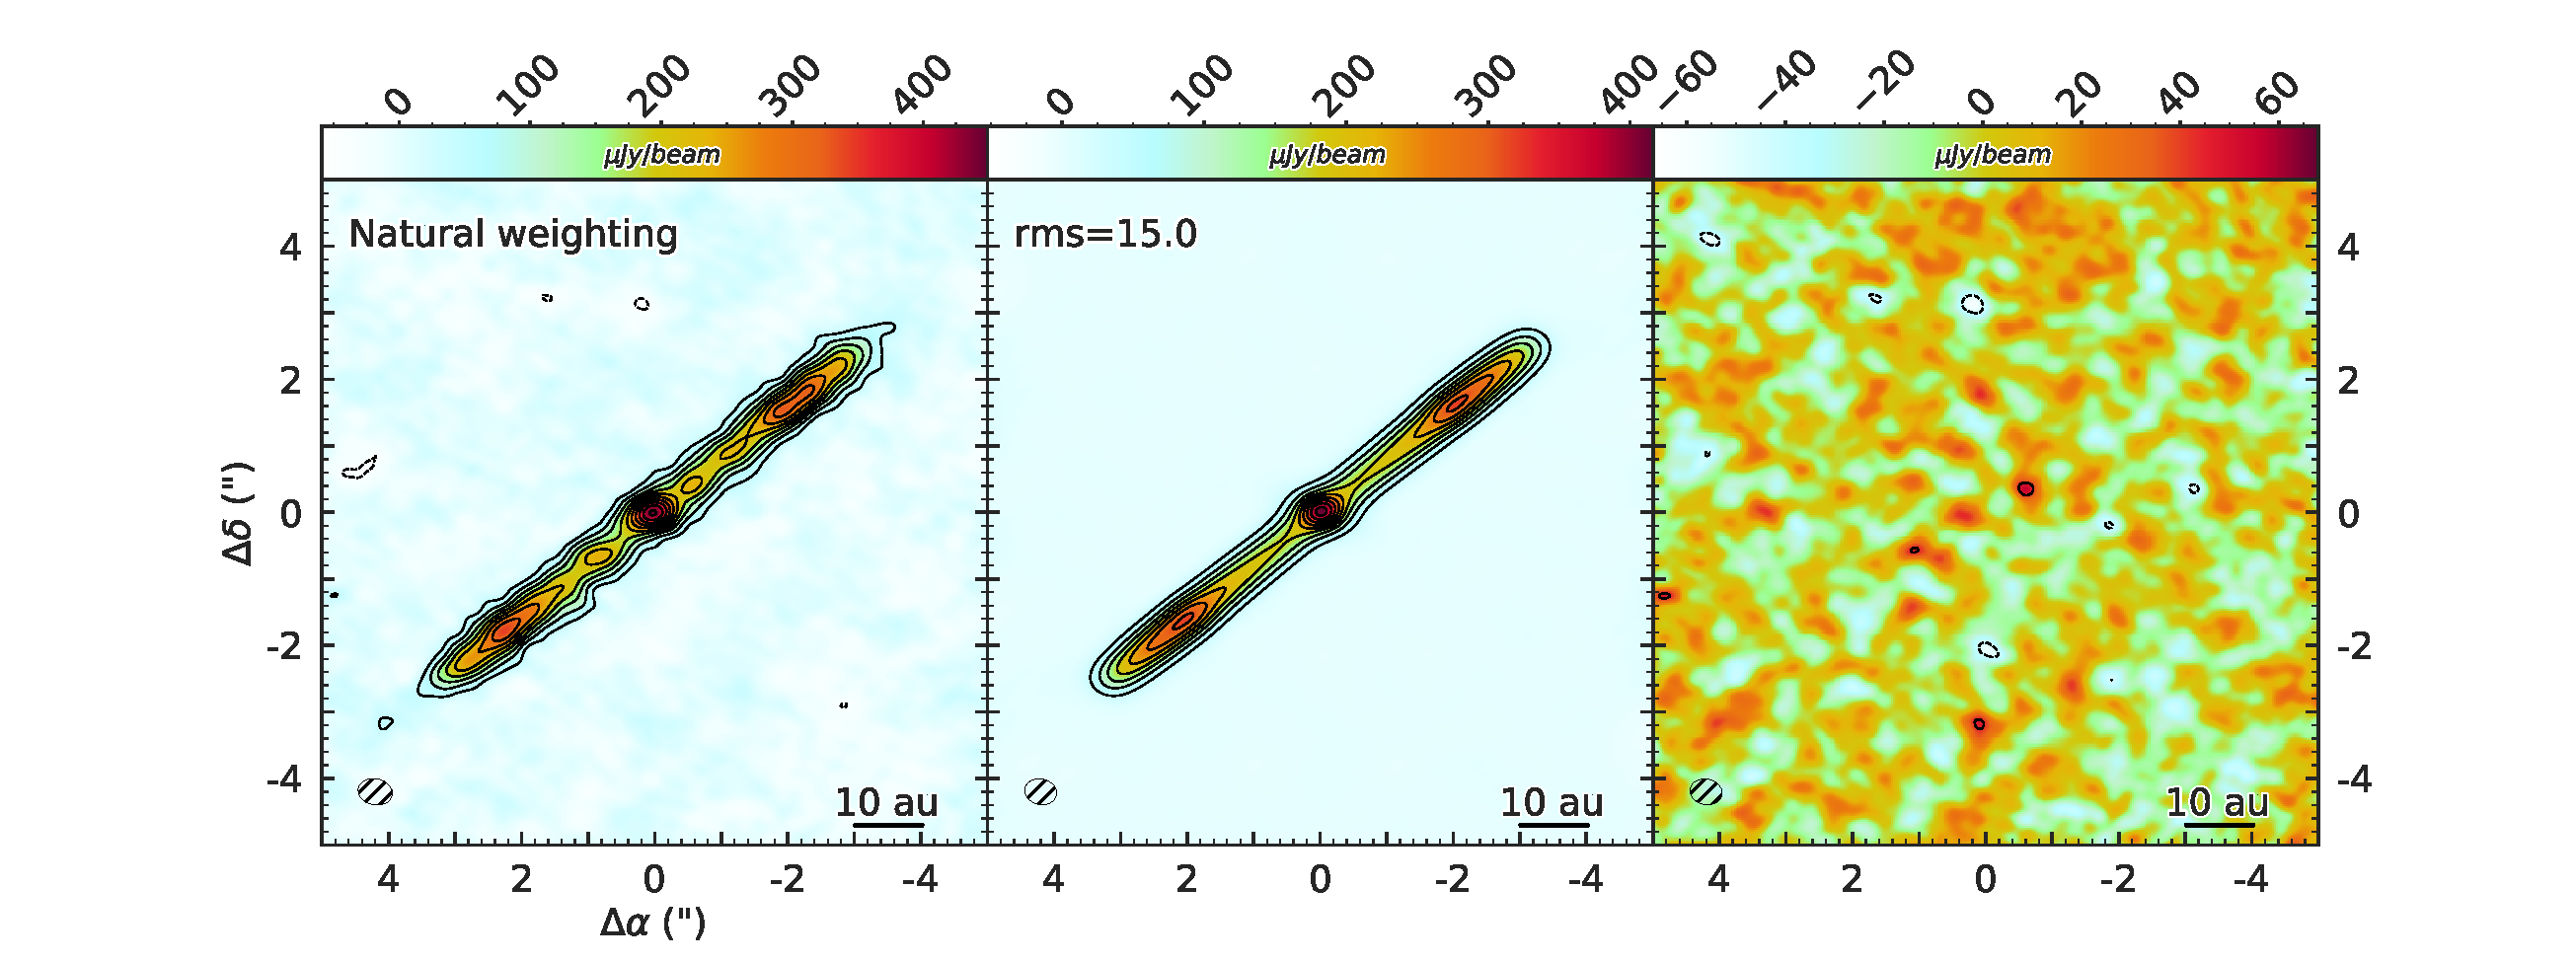
\includegraphics[width=\linewidth]{run6_bestfit_global_concise}
  \caption{(left to right) ALMA observations of AU Mic, best fit model, and best fit model residuals. Contours are integer multiples of 3$\sigma$.}
  \label{fig:bf}
\end{figure}

This summer we've been investigating the vertical and radial structure of AU Mic using MCMC methods. 
Most parameters are well behaved, but a few questions remain:
  
The posterior for inner radius exhibits bimodality, with one solution at $\sim 8$ au and another at $\sim 20$ au. 
We will be implementing a gap to see how it affects this bimodality, also motivated by the morphology of the data and residuals at $\sim 1"/10$ au.
  
Additionally, we are investigating the spatial scales to which our data our sensitive| models with both linear and constant scale height prescriptions prefer values for scale height that do not seem to be lower limits (see Figure \ref{fig:kde}).
We are fixing the scale factor to a value an order of magnitude below our resolution limits in order to compare a spatially unresolved model to our best-fit resolved model and clarify what features of the data favor a resolved scale height.

\begin{figure}[h]
  \centering
  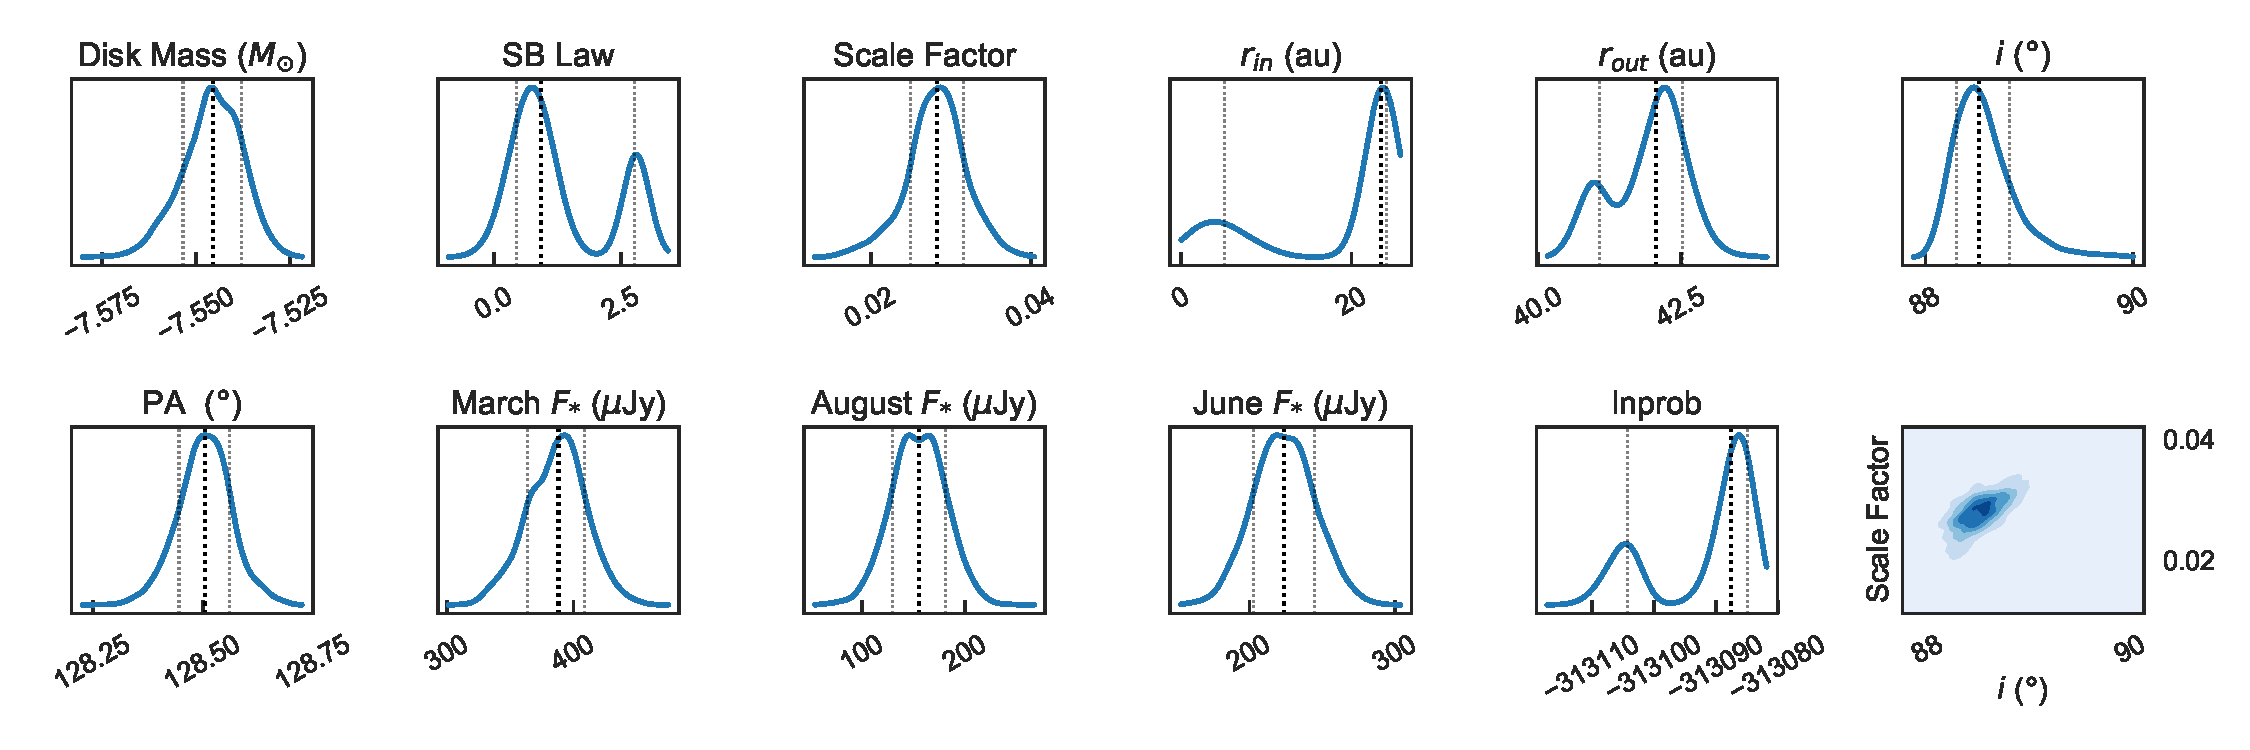
\includegraphics[width=\linewidth]{run6_kde}
  \caption{Posterior distribution of free parameters. The outer dotted lines designate the 16th and 84th percentiles, while the inner line designates the median. The bottom right plot shows the posterior relationship between scale factor and inclination; this degeneracy motivated us to try a model with constant scale height.}
  \label{fig:kde}
\end{figure}



\end{document}
